\documentclass[a4paper,11pt]{article}

\usepackage[spanish,es-nodecimaldot]{babel}
\usepackage[utf8]{inputenc}
\usepackage[T1]{fontenc}
\usepackage{amsmath,amssymb}
\usepackage{graphicx}
\usepackage{booktabs}
\usepackage[margin=2.5cm]{geometry}
\usepackage[hidelinks]{hyperref}

\graphicspath{{figures/}}

\title{Criterio de interacción basado en la superposición celular}
\author{}
\date{}

\begin{document}
	
	\maketitle
	
	\section{Superposición y criterio de interacción}
	
	Para definir que dos células interactúen, proponemos un criterio basado en la superposición celular. En particular, nos vamos a centrar en células redondas (con relación de aspecto $\phi=1$) y elongadas con $\phi=2.7$.
	
	Para formas y orientaciones fijas, y una dirección de acercamiento determinada, la superposición gaussiana puede escribirse como
	
	\begin{equation}
		I_{ij}(r)
		=
		I_{ij}^{\max}
		\exp\left(-q_{ij}r^2\right),
		\qquad q_{ij}>0.
	\end{equation}
	Aquí, $r$ es la distancia entre centros,
	$I_{ij}^{\max}$ es la superposición con centros coincidentes
	para esas mismas formas y orientaciones, y $q_{ij}$
	incorpora la geometría del par y la dirección de acercamiento.
	
	Definimos la superposición normalizada como
	\begin{equation}
		\xi_{ij}(r)
		=
		\frac{I_{ij}(r)}{I_{ij}^{\max}}
		=
		\exp\left(-q_{ij}r^2\right).
	\end{equation}
	Esta cantidad permite comparar pares mediante una misma
	fracción de su superposición máxima. No representa la
	fracción de área compartida por sus contornos.
	
	Para dos células redondas idénticas,
	\begin{equation}
		\xi(r)
		=
		\exp\left(-\frac{r^2}{4R^2}\right).
	\end{equation}
	En el contacto geométrico, $r=2R$, se obtiene
	$\xi=e^{-1}$. El mismo resultado se cumple para dos células
	elongadas idénticas y alineadas que se acercan por un eje
	principal: basta reemplazar $R$ por el semieje correspondiente.
	
	Esto motiva el criterio
	\begin{equation}
		\boxed{
			i \text{ y } j \text{ interactúan}
			\quad\Longleftrightarrow\quad
			\xi_{ij}>e^{-1}.
		}
		\label{eq:interaction}
	\end{equation}
	Para cada configuración, la frontera de interacción se
	encuentra entonces en
	\begin{equation}
		r_{\mathrm{cut}}
		=
		\sqrt{\frac{-\ln(e^{-1})}{q_{ij}}}
		=
		\frac{1}{\sqrt{q_{ij}}}.
	\end{equation}
	
	\section{Interpretación de las figuras}
	
	La figura~\ref{fig:overlap} compara la superposición absoluta
	y normalizada en función de la distancia entre centros.
	En el panel izquierdo, los máximos dependen de la
	configuración. En el derecho, todas las curvas parten de
	uno, conservando su distinta dependencia con la distancia.
	
	Los puntos señalan la frontera de interacción
	$r_{\mathrm{cut}}$, no necesariamente el contacto geométrico.
	Por construcción, todos se encuentran a la altura
	$\xi=e^{-1}$ en el panel normalizado. Sus alturas en el
	panel absoluto son $I_{ij}^{\max}e^{-1}$.
	
	\begin{figure}[htbp]
		\centering
		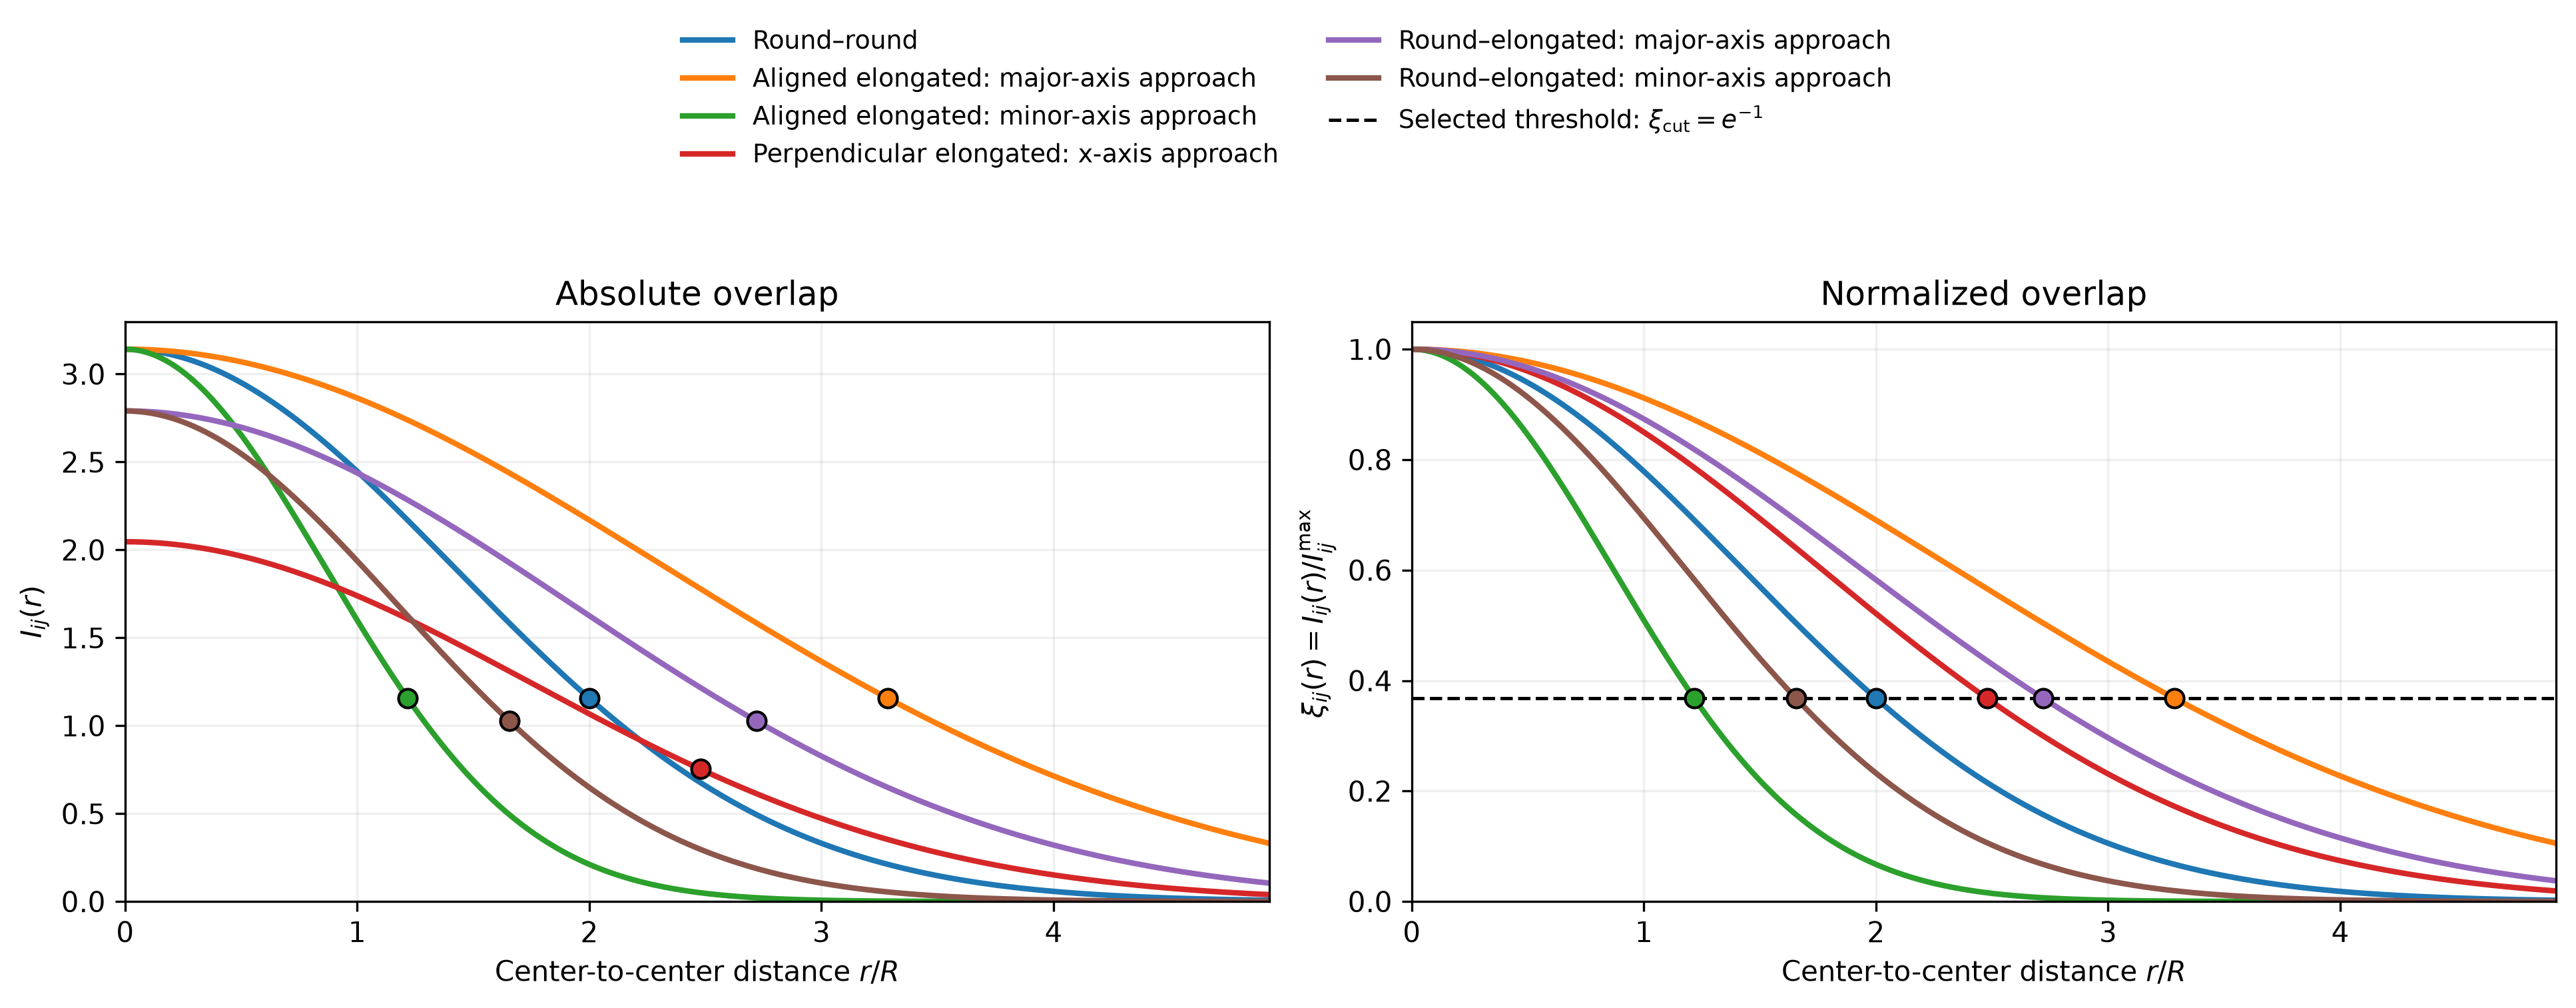
\includegraphics[width=\textwidth]{../figures/pairwise_overlap.png}
		\caption{
			Superposición absoluta y normalizada para distintos
			pares y direcciones de acercamiento.
			Los puntos indican dónde se alcanza el umbral elegido.
			Para cada curva, las separaciones menores que ese valor
			corresponden a pares que interactúan.
			Las curvas se muestran completas para visualizar
			también la superposición fuera del alcance seleccionado.
		}
		\label{fig:overlap}
	\end{figure}
	
	Para evaluar la correspondencia con el contacto real entre
	los contornos, la figura~\ref{fig:contact} utiliza la distancia
	reescalada $r/r_{\mathrm{contact}}$. Por lo tanto, todos los
	pares se tocan en $r/r_{\mathrm{contact}}=1$.
	
	Los círculos muestran la superposición normalizada al
	contacto, mientras que las cruces indican la separación
	a la que se alcanza el umbral. Si ambos coinciden, el
	criterio reproduce exactamente el contacto. Una cruz a
	la derecha de uno indica que se admite interacción entre
	contornos todavía separados.
	
	\begin{figure}[htbp]
		\centering
		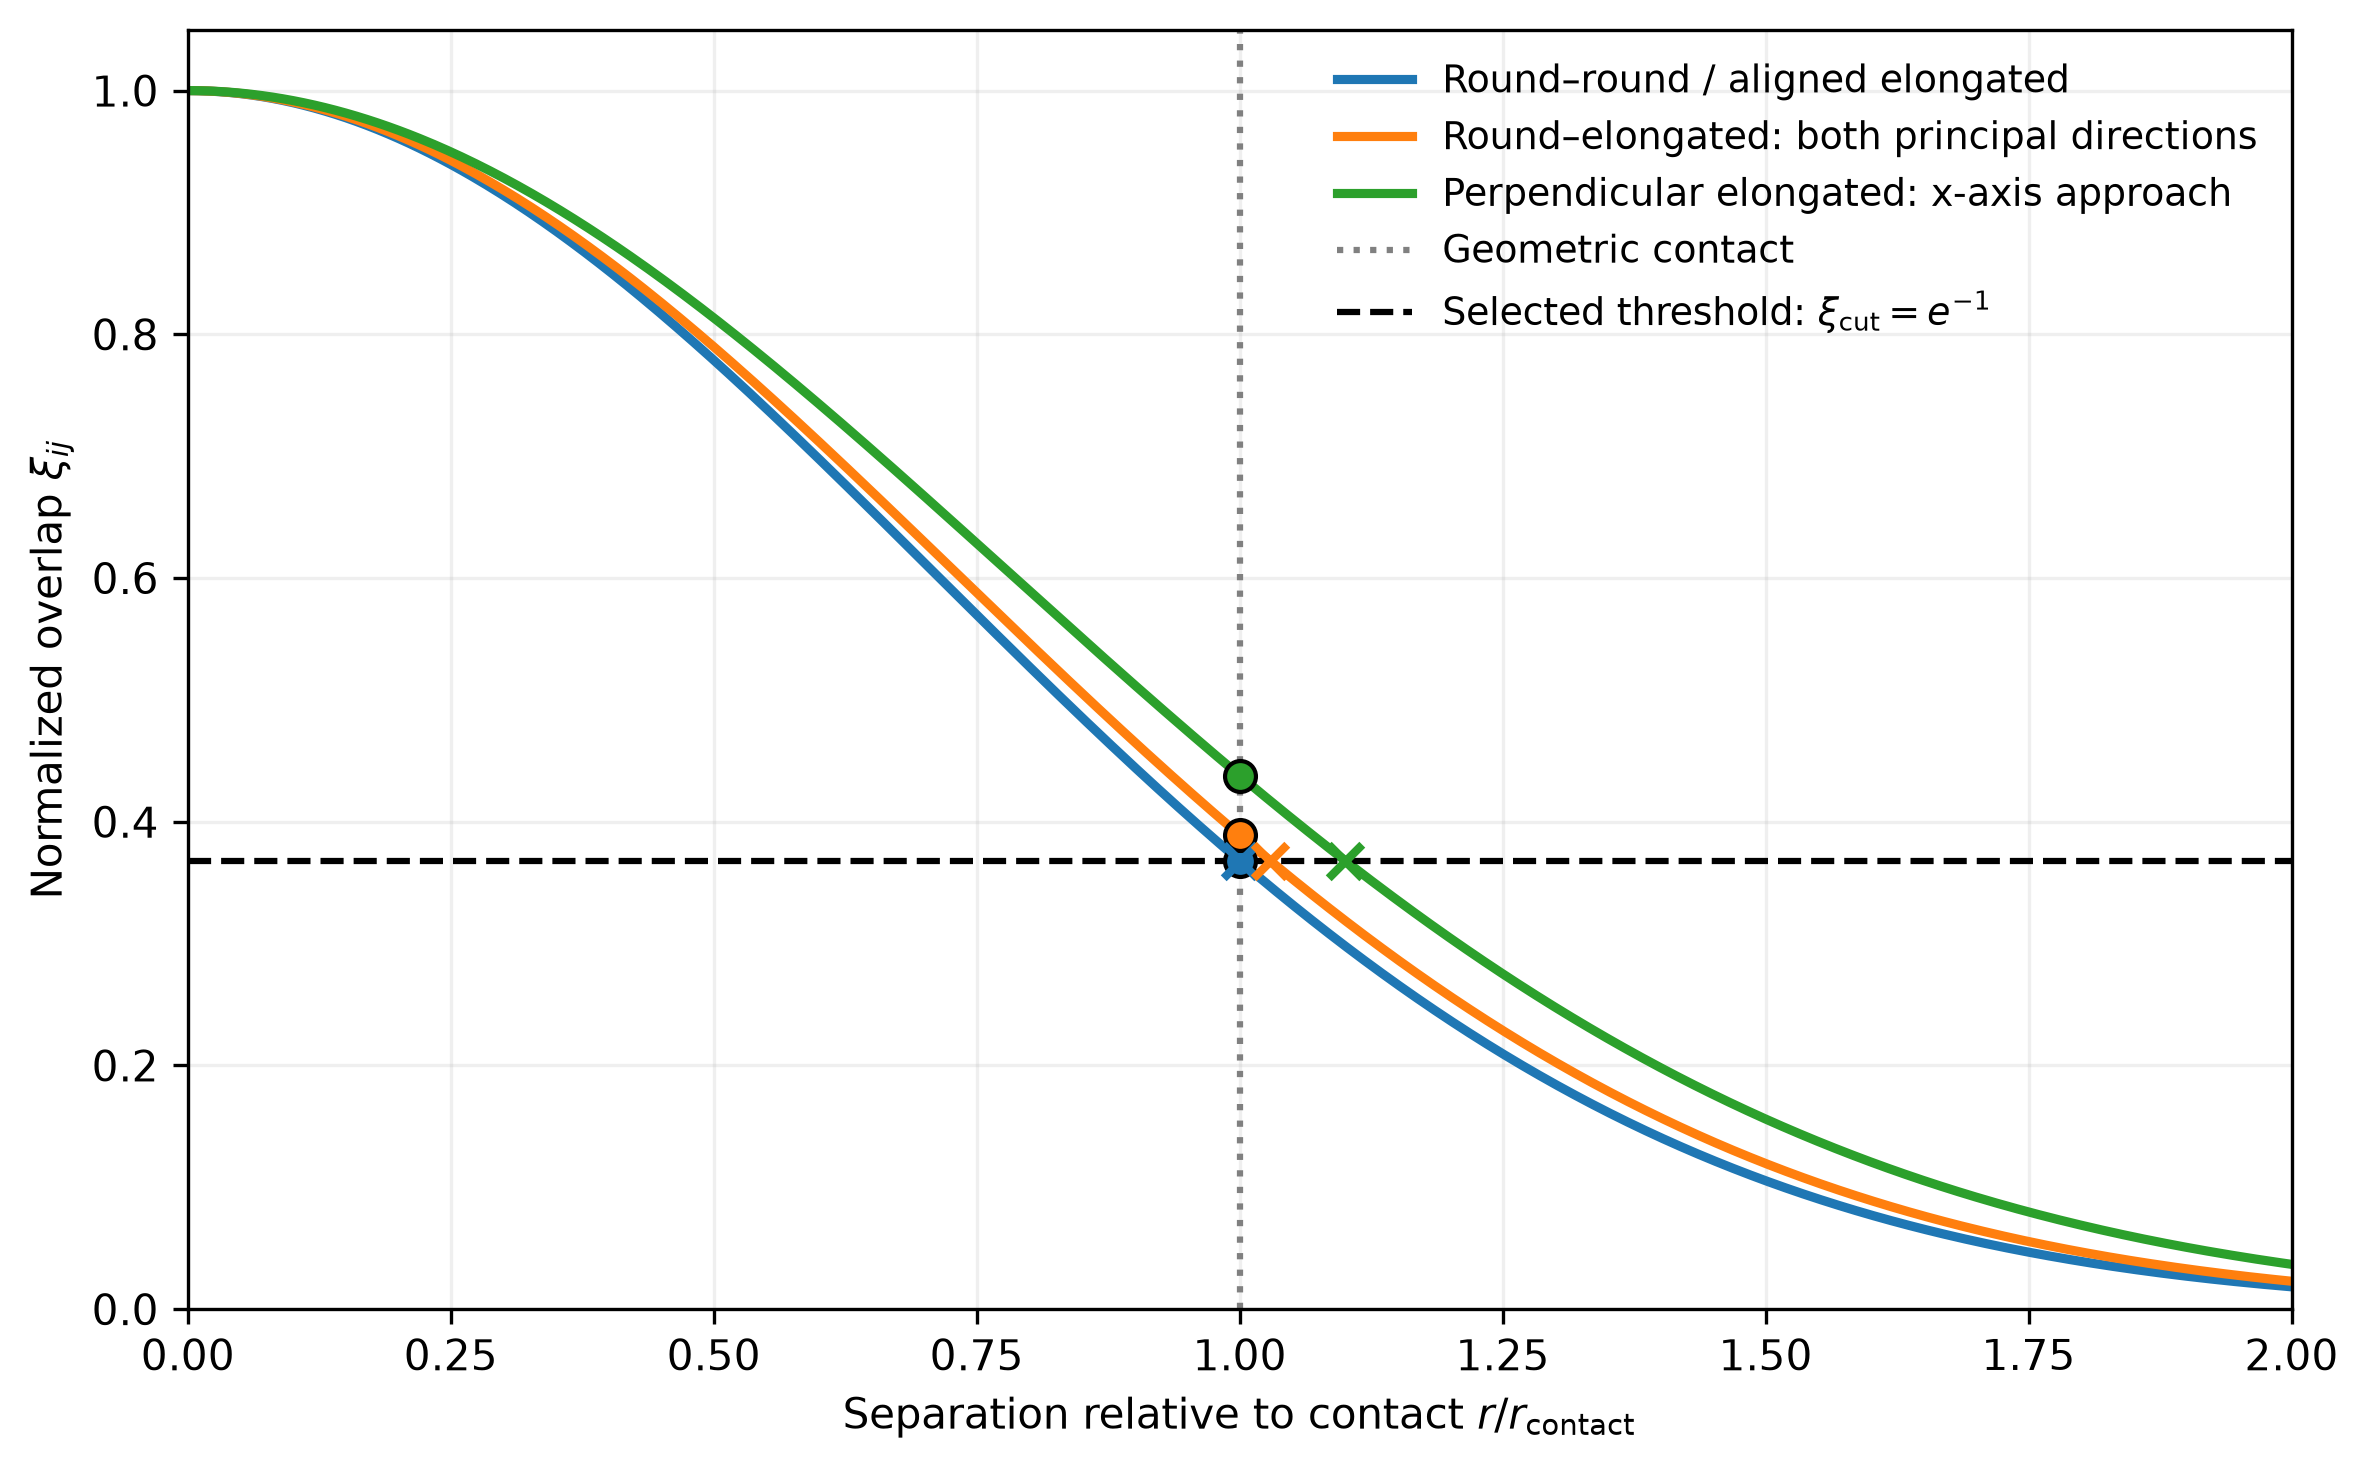
\includegraphics[width=0.78\textwidth]{
			../figures/overlap_relative_to_contact.png
		}
		\caption{
			Superposición normalizada en función de la separación
			relativa al contacto geométrico.
			Los círculos marcan el contacto y las cruces la
			frontera de interacción.
			Las configuraciones cuyas curvas reescaladas coinciden
			se muestran agrupadas.
		}
		\label{fig:contact}
	\end{figure}
	
	Para las configuraciones examinadas, los resultados son:
	
	\begin{center}
		\begin{tabular}{lcc}
			\toprule
			Configuración
			& $\xi(r_{\mathrm{contact}})$
			& $r_{\mathrm{cut}}/r_{\mathrm{contact}}$ \\
			\midrule
			Redondas o elongadas idénticas alineadas
			& $0.3679$ & $1.000$ \\
			Redonda--elongada, por los ejes principales
			& $0.3890$ & $1.029$ \\
			Elongadas perpendiculares, acercamiento en $x$
			& $0.4379$ & $1.101$ \\
			\bottomrule
		\end{tabular}
	\end{center}
	
	El criterio reproduce el contacto en el primer grupo y
	permite un alcance aproximadamente un $3\%$ y un $10\%$
	mayor en los otros dos. Estos valores corresponden a
	las configuraciones estudiadas; no constituyen cotas
	para orientaciones arbitrarias.
	
	\section{Elección para el modelo}
	
	Adoptamos $\xi_{\mathrm{cut}}=e^{-1}$ como un criterio de
	proximidad dependiente de la forma y orientación, con una
	referencia geométrica explícita. Su propósito es definir
	el alcance de interacción del modelo, sin exigir que
	coincida exactamente con el contacto en toda configuración. No imponemos un corte adicional basado en la suma de semiejes mayores, excepto por la condición dada por la búsqueda en la grilla.
	
	Utilizamos el mismo umbral para aceptar elongaciones:
	la posición y forma propuestas son admisibles únicamente si
	\begin{equation}
		\xi_{ij}^{\mathrm{propuesta}}\leq e^{-1}
		\qquad
		\text{para todo } j\neq i.
	\end{equation}
	Así, una elongación no introduce pares por encima del umbral de interacción en la configuración propuesta.
	
\end{document}